

\section{Experiment Results}


\begin{figure*}[ht!]%
    \centering
    \subfloat[3s\_vs\_5z (hard)]{
        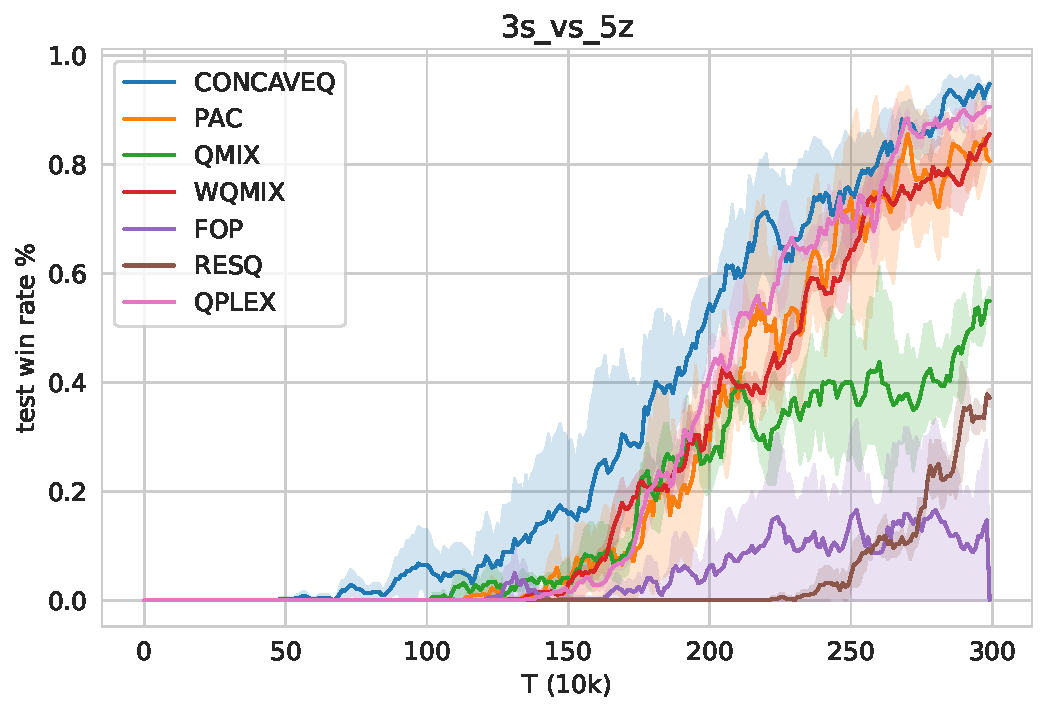
\includegraphics[width=0.33\linewidth]{new_figure/3s_vs_5z_win_rate_comp_300_tab10_0628.pdf}
        }%\hfill
    \subfloat[5m\_vs\_6m (hard)]{
        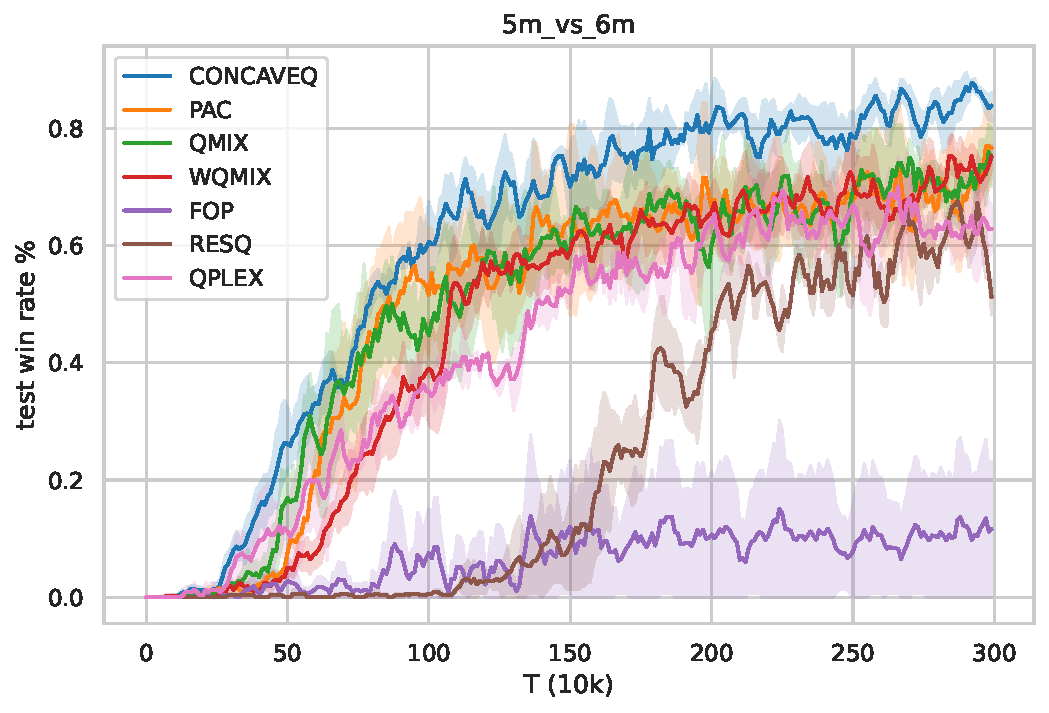
\includegraphics[width=0.33\linewidth]{new_figure/5m_vs_6m_win_rate_comp_300_tab10_0628.pdf}
        }%\hfill
    \subfloat[27m\_vs\_30m (Super hard)]{
        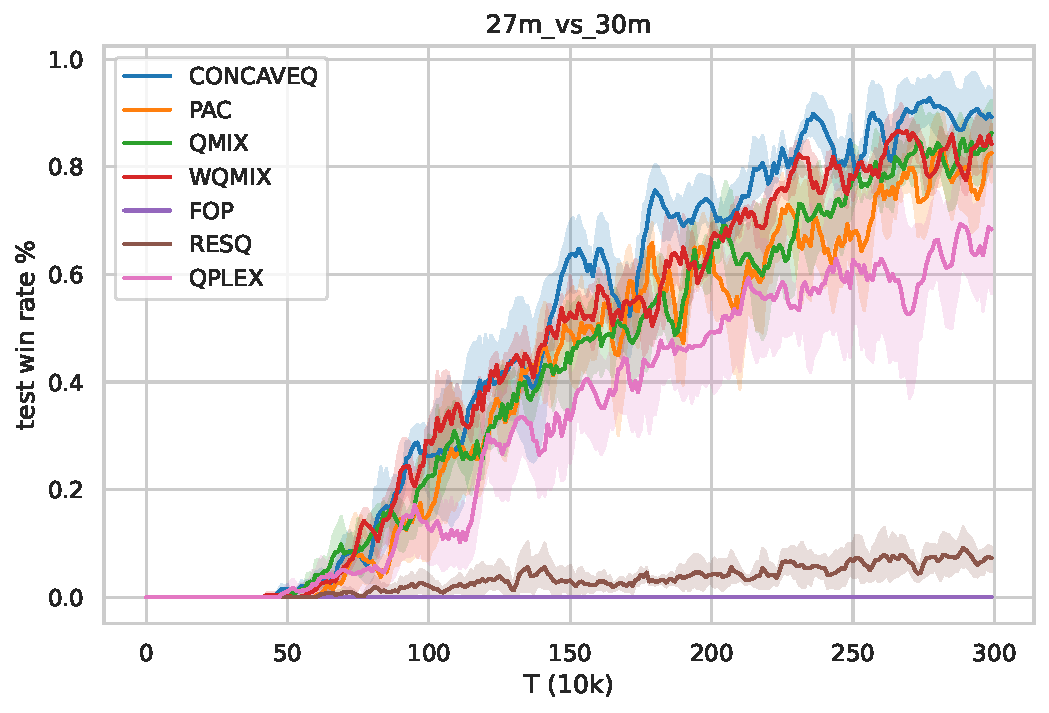
\includegraphics[width=0.33\linewidth]{new_figure/27m_vs_30m_win_rate_comp_300_tab10_0628.pdf}
        }\\
        \subfloat[6h\_vs\_8z (Super hard)]{
        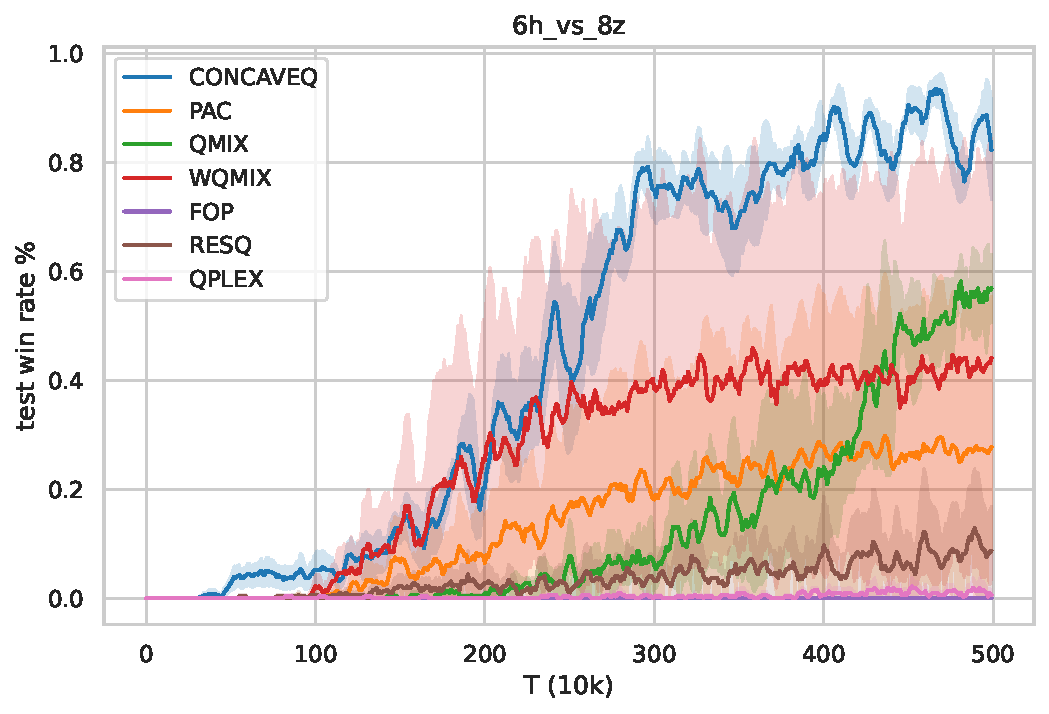
\includegraphics[width=0.33\linewidth]{new_figure/6h_vs_8z_win_rate_comp_500_tab10_0628.pdf}
        }%\hfill
        \subfloat[Corridor (Super hard)]{
        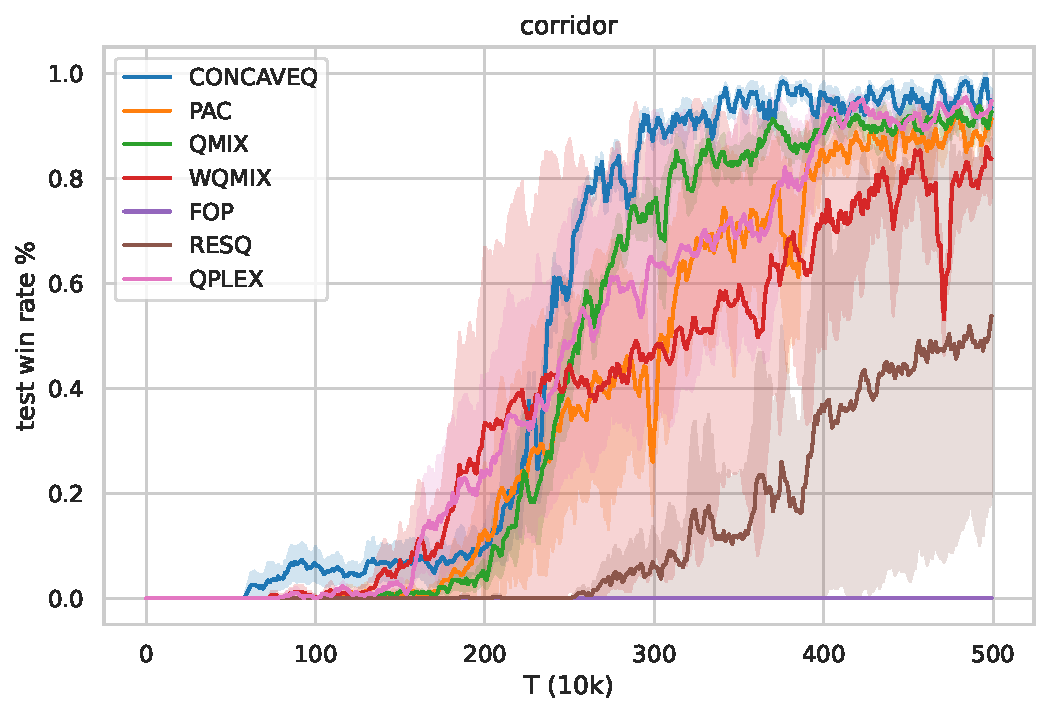
\includegraphics[width=0.33\linewidth]{new_figure/corridor_win_rate_comp_500_tab10_0628.pdf}
        }%\hfill
    \subfloat[MMM2 (Super hard)]{
        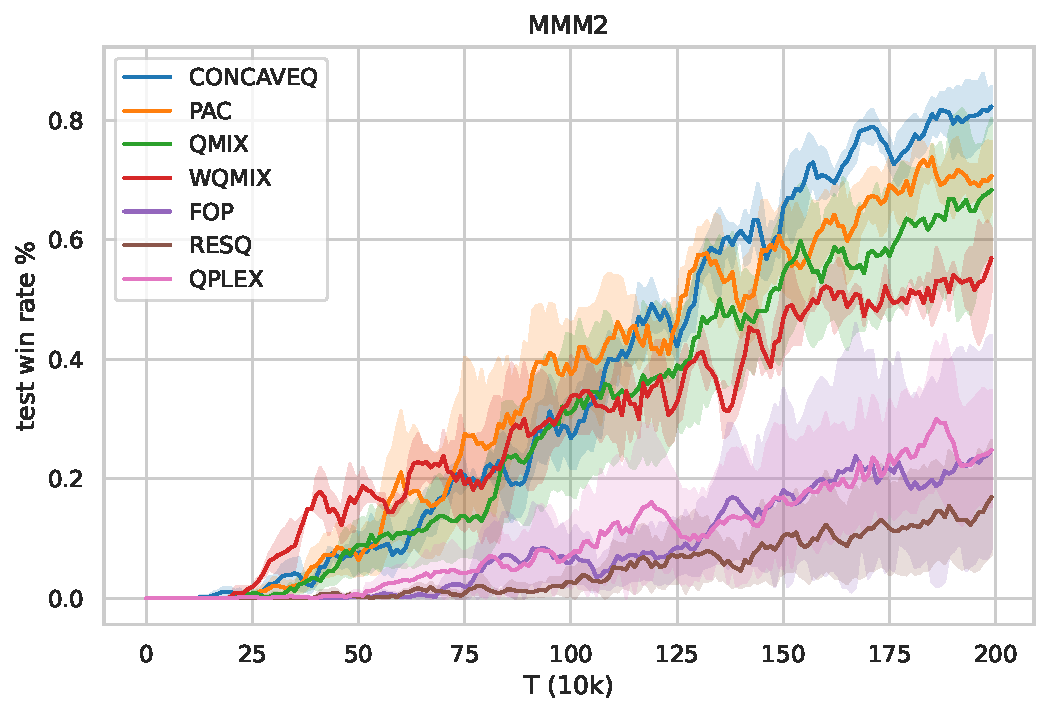
\includegraphics[width=0.33\linewidth]{new_figure/MMM2_win_rate_comp_200_tab10_0628.pdf}
        }\\    
    \caption{Average test win rate on the SMAC tasks.}
    \label{exp_smac}
% \end{figure}
\end{figure*}
In this section, we present our experimental results with the state-of-the-art methods on Predator-Prey and the StarCraft II Multi-Agent Challenge (SMAC)\cite{samvelyan2019starcraft}. For fair evaluations, the hyper-parameters of all algorithms under comparison as well as the optimizers are the same. Each experiment is repeated 3 times with different seeds. The presented curves are smoothed by a moving average filter with its window size set to 5 for better visualization. More implementation details and experimental introduction and settings can be found in the Appendices. 


\subsection{Predator Prey}
Predator-Prey is a complex partially observable multi-agent environment, where  8 agents cooperate as predators to hunt 8 prey within a  $10 \times 10$ grid. If two or more adjacent predator agents carry out the \textit{catch} action simultaneously, it is a  successful catch and the agents receive a reward $r = 10$. A failed attempt where only one agent captures the prey will receive a punishment reward $p \leq 0$. The more negative $p$ is, the higher level of coordination is needed for the agents. 



We select multiple state-of-the-art MARL approaches as baseline algorithms for comparison, which includes value-based factorization algorithms (i.e., QMIX in \cite{QMIX}, WQMIX in \cite{WQMIX}, PAC in \cite{pac},  QPLEX in \cite{QPLEX}, and RESQ in \cite{ResQ}), and decomposed actor-critic approaches (i.e., FOP \cite{fop} ).  
Fig~\ref{exp_stag_hunt} shows the performance of our scheme and the six baselines when punishment $p$ varies from $0$ to $-2$, in which the $x$-axes and $y$-axes represent the number of training episodes and the test mean rewards, respectively. According to the curves in Fig~\ref{exp_stag_hunt}, the following results can be observed. (1) When $p=0$,  CONCAVEQ, PAC, WQMIX, and QMIX can learn good policies and obtain the highest reward when they have been trained for more than $50$ episodes. In other words, the performance of our algorithm is as good as the state-of-the-art works. (2) When punishment gets larger, i.e. $p=-0.5, p= -1.5$ and $p=-2.0$, only CONCAVEQ and WQMIX can still achieve high rewards within $60$ episodes while CONCAVEQ is able to converge faster than WQMIX, the others gradually fail due to their monotonicity constraints or representational limits. These results demonstrate CONCAVEQ's ability in challenging cooperative MARL tasks that require non-monotonic action selections.





\subsection{StarCraft II Multi-Agent Challenge (SMAC)}
In SMAC, agents are divided into two teams to cooperate with allies and compete against enemies or against the other team controlled by the built-in game AI. In the simulation, the agents act according to their local observations and learning experiences.


Note that the state-of-the-art algorithms have already achieved a very good performance on the easy and medium maps, which makes it difficult to present clear comparisons and potential improvements. We carry out our experiment in six maps consisting of two hard maps (\texttt{3s\_vs\_5z, 5m\_vs\_6m}) and four super-hard maps (\texttt{ 27m\_vs\_30m, 6h\_vs\_8z, MMM2, corridor}). The baseline algorithms are the same as those in the Predator-Prey environment. 


Details of the environment setting and other training details like network hyperparameters can be found in Appendices.

The performance of our algorithm and the baselines in those hard and super hard maps are presented in Figure \ref{exp_smac}, in which the $x$-axes and $y$-axes represent the number of training episodes and the test win rate, respectively. For almost all scenarios, we found that our algorithm is able to converge faster and deliver a higher win rate. Especially on the \texttt{6h\_vs\_8z} map CONCAVEQ significantly outperforms other baselines by a large margin. We note that the \texttt{6h\_vs\_8z} map requires a sophisticated strategy to take the win, where one unit will be drawing firepower from the enemy units while circling around the edge of the map so the rest friendly units can deliver damages. This implies CONCAVEQ imposes a higher capability of exploration and function representational abilities.





\subsection{Ablation Studies}
We carry out ablation experiments to demonstrate the effectiveness and contribution of each core component introduced in CONCAVEQ on 3s\_vs\_5z scenario in SMAC. As shown in Fig.\ref{exp_ablation} we consider verifying the effect of (1) concave mixing network by replacing it with 4-layer monotonic network as \textit{CONCAVEQ\_linear},  (2) iterative action selection which removes the iterative procedure as \textit{CONCAVEQ\_no\_iter}, (3) soft policy network which removes the soft policy network as \textit{CONCAVEQ\_no\_policy},  (4) disable both iterative action selection and soft policy network as \textit{CONCAVEQ\_disabled}, (5) further remove the central $Q^*$ as \textit{CONCAVE\_no\_$Q^*$}. The results show that CONCAVEQ overperforms these ablated versions. \textit{CONCAVEQ\_no\_iter} has lower rewards than \textit{CONCAVEQ} due to a lack of iterative action selection which is unfavorable to finding the optimal actions. Removing the soft policy network also leads to a performance drop due to a lack of a proper action selection scheme during execution.  The reward of \textit{CONCAVEQ\_linear} grows slowly at first as linear layers have weaker representation ability than concave mixing networks.  \textit{CONCAVEQ\_no\_$Q^*$} suffers from the most significant performance drop after most core components are removed from the original design. Such results validate how each component is crucial for achieving performance through experiments. 

\setlength\intextsep{0pt}
\begin{figure}
\centering
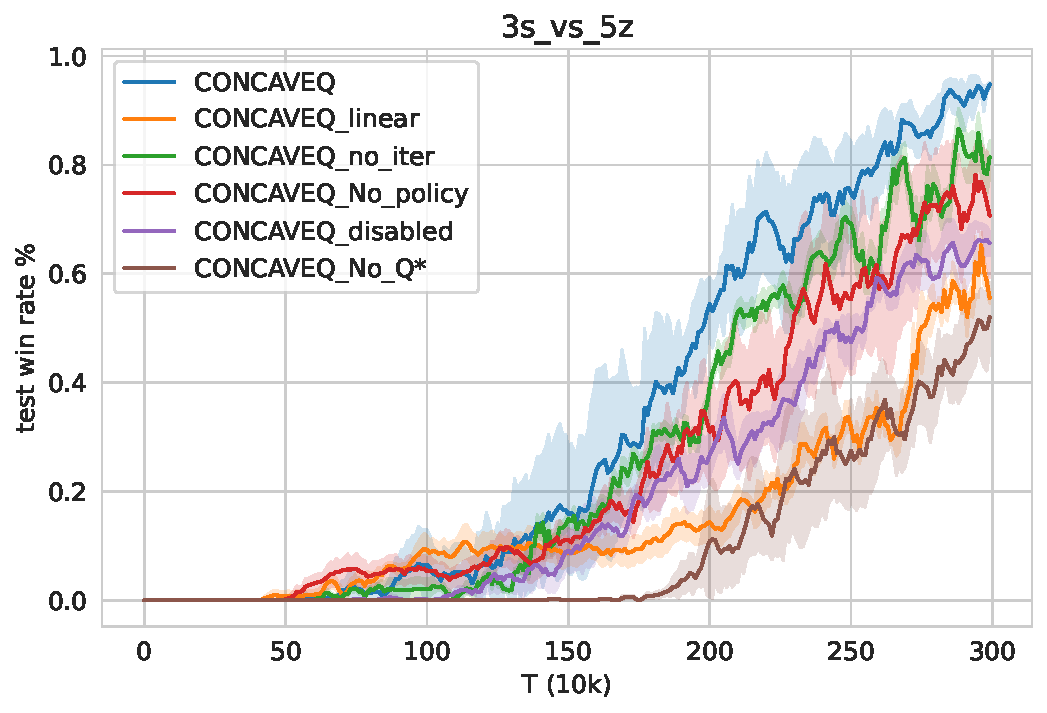
\includegraphics[width=0.45\textwidth]{new_figure/3s_vs_5z_win_rate_comp_300_tab10_ablation.pdf}
\caption{Ablations results comparing CONCAVEQ and its  ablated versions on SMAC map \texttt{3s\_vs\_5z}}
\label{exp_ablation}
\end{figure}

